\chapter{Analyzing  data with regard to Customer Satisfaction}
\label{ch:implementation}

This chapter focuses on the design and implementation of approaches to analyze the data made available by the case study and build a solution to make predictions about customer satisfaction based on available usage data. The implementation relies on ideas which were introduced and described in more detail within the previous chapter. 

\section{Overview on available data}
Before diving into the details of the proposed approach, it will be briefly pointed out how much data at Tractive could be provided, which data sources were available for the practical part of this thesis and how they are technologically represented. 

Although offering some miscellaneous apps and hardware accessories, the main focus of Tractive is selling a GPS device to allow customers to track their pets on a smartphone or in the web. The work in this thesis focused on data produced by customers of the GPS device. Due to the reason that this product is very versatile, data flows into the system from different sources. Data is generated by the hardware device itself, by the customers relationship with the company over time or the usage of provided software products (smartphone- and web app) and their functionalities, to name the important sources.

From a technological perspective, in order to manage this data, a persistent semi-structured database, namely MongoDB, is used. Following listing outlines essential metrics regarding this database to give the reader some understanding about the dimensions.

\begin{itemize}
	\item Infrastructure: 6 nodes with MongoDB server whereby data is horizontally distributed among 5 clusters (in MongoDB also called shards). This ensures high availability even if a database node goes down or a shard becomes unavailable.
	\item Databases: The whole DBMS (Database Management System) is split into a main database, containing all raw and transactional data, and a metrics database which contains aggregated data like KPIs (Key Process Indicators) and analytical relevant data. 
	\item Number of collections: 66
	\item Number of customers actively (i.e. paying for the subscription) using a device: 78038 (as of 26.11.2017 09:58 UTC+1)
\end{itemize}

Besides this database, a relevant point, especially when it comes to customer satisfaction, is the contact of customers with the company internal support service, as already indicated by the customer satisfaction model in figure \ref{fig:satisfactionModel}. The support service of Tractive uses a third party software, called Zendesk, to handle customer concerns. This data is managed completely by Zendesk. With regard to the implementation, the author considered to use the official API (Application Programmer Interface) in order to fetch relevant data about customer interactions. 

\section{Identification of relevant data sources}
\label{sec:dataSources}
On the one hand, statistical analysis and data-driven approaches are rich tools to gain new insights into the data and find hidden associations and relationships but on the other hand these approaches will not deliver any satisfying results if they work with wrong or invalid datasets as input. Therefore it is essential to invest enough resources on selecting relevant data sources and ensuring high quality within this data before starting with any analytical approach. Considering right and valid data was not only mentioned once in literature as a key factor for successful data analysis \cite{neckel2015}. 

\subsection{Selecting the right data based on its representativeness regarding Customer Satisfaction}
The approach this thesis followed for selecting relevant data sources is based on the definition of customer satisfaction as it was modeled in section~\ref{sec:custSatisfactionDefinition}. Furthermore, as already indicated in section~\ref{ssec:custSatTheories}, the focus is on the provided service quality and observed performance yielded due to customer behavior, since these metrics can be represented in data and as a result are measurable. In order to create a list of all relevant data collections, the author started with a summarization of properties and features of the Tractive GPS device which are advertised actively to potential customers. As representative resource the landing web page of the company, namely https://tractive.com plus the necessary sub pages with information about the Tractive GPS device, were used to extract this information. The website is the major source of customer conversion and lists all relevant characteristics and features of the product. Figure \ref{fig:tractiveLanding} shows an extract of the home page.

\begin{figure}
	\centering
	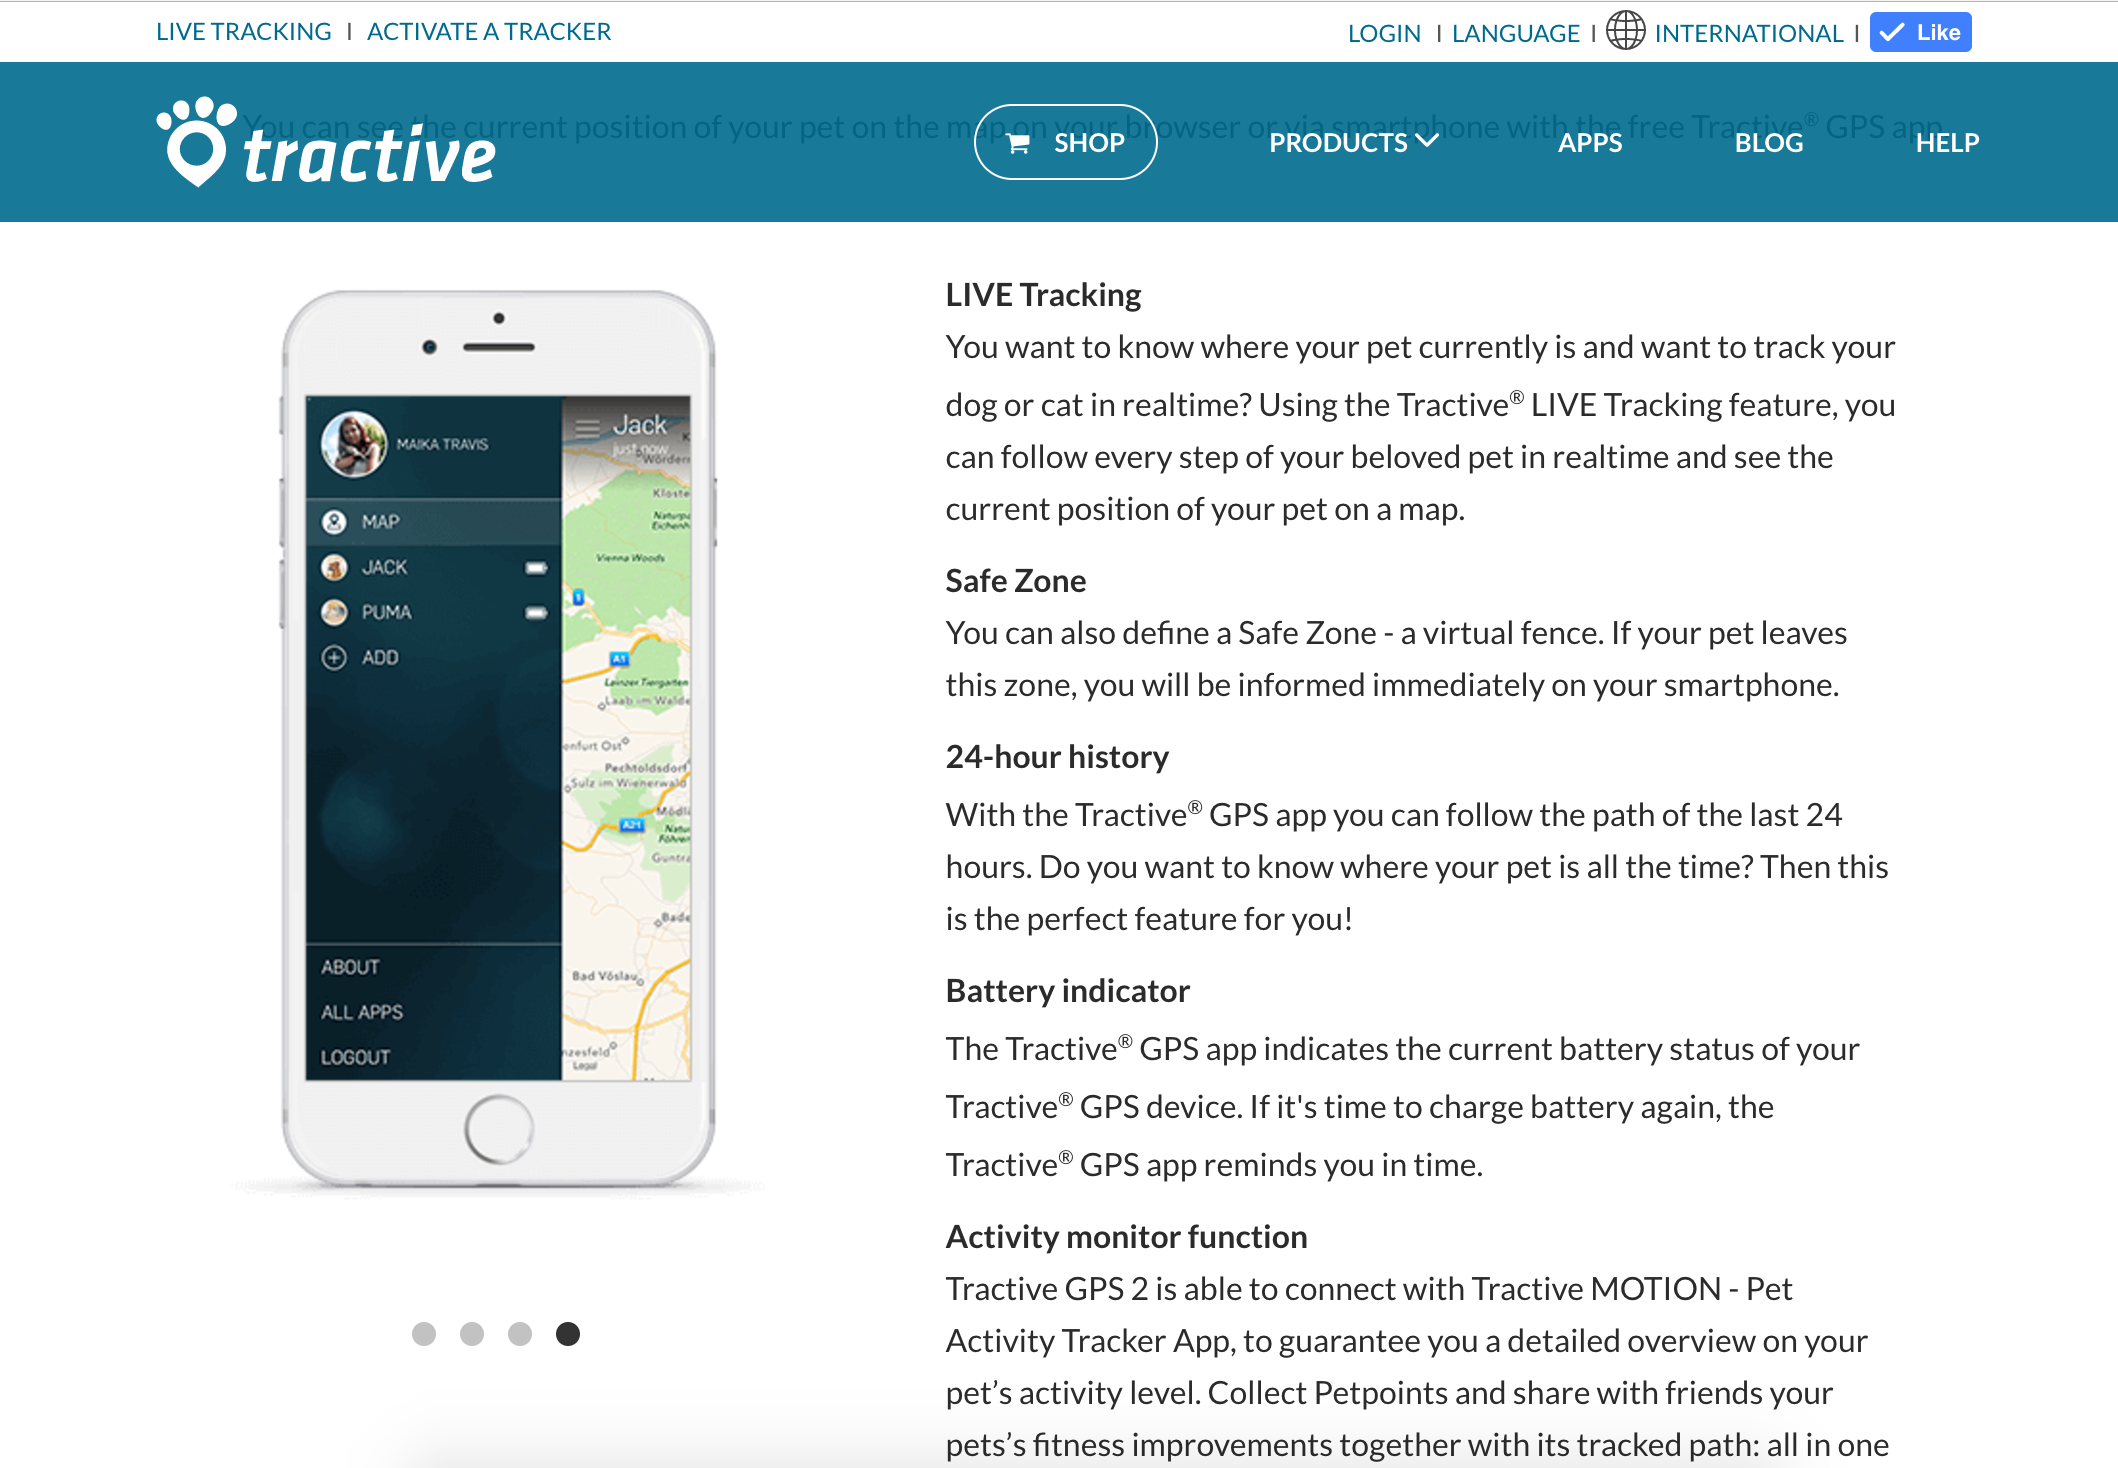
\includegraphics[width=1.0\textwidth]{img/tractiveLanding.png}
	\caption{Extract of landing page https://tractive.com}
	\label{fig:tractiveLanding}
\end{figure} 

Other sources used in marketing like social media channels provide brief summarizations and link to the website. Therefore it can be implied that product descriptions on the landing web page are decisive for customers and drive their expectations with regard to the product. Table~\ref{tab:productFeatures} gives an overview on important properties and features regarding Tractive GPS from a customers perspective. Moreover, it assigns the data which considered as useful for reasoning about customer satisfaction, i.e. it indicates what a customer can expect when he or she purchases the product.

\begin{table}[]
	\centering
	\resizebox{\textwidth}{!}{%
		\begin{tabular}{|l|l|l|}
			\hline
			\multicolumn{1}{|c|}{\textbf{Feature / Characteristic}} & \multicolumn{1}{c|}{\textbf{Description}} & \multicolumn{1}{c|}{\textbf{\begin{tabular}[c]{@{}c@{}}Nature of data suitable for \\ predicting customer satisfaction\end{tabular}}} \\ \hline
			Locate pet anytime, anywhere & \begin{tabular}[c]{@{}l@{}}See location of pet accurately \\ on a map on the Smartphone\end{tabular} & Position data (GPS, Mobile Cell) \\ \hline
			Live Tracking & \begin{tabular}[c]{@{}l@{}}Follow the trace of a pet in \\ realtime on a smartphone\\ or on a web page\end{tabular} & Live Tracking commands statistics \\ \hline
			Virtual fences & \begin{tabular}[c]{@{}l@{}}Creating a virtual fence and \\ get notified if pet leaves \\ selected safe area\end{tabular} & \begin{tabular}[c]{@{}l@{}}Number of times pet leaves \\ and enters virtual fence,  \\ reliability data regarding notifications\end{tabular} \\ \hline
			Battery indication & \begin{tabular}[c]{@{}l@{}}If battery of GPS device is \\ full or is nearly empty, \\ it will be indicated \\ in the Smartphone app\end{tabular} & \begin{tabular}[c]{@{}l@{}}Reliability of data regarding \\ battery notifications\end{tabular} \\ \hline
			Integrated light & \begin{tabular}[c]{@{}l@{}}Customers can turn on the \\ integrated LED (Light-Emitting Diode) \\ on the GPS device \\ via the Smartphone\end{tabular} & LED command statistics \\ \hline
			100\% waterproof & \begin{tabular}[c]{@{}l@{}}A product characteristic \\ customers trust in, since many \\ pets often get wet\end{tabular} & \begin{tabular}[c]{@{}l@{}}Hardware defects due to \\ water damage\end{tabular} \\ \hline
			Premium Customer Service & \begin{tabular}[c]{@{}l@{}}With a premium service plan, \\ it is promised that customers \\ get feedback within 24 hours \\ on weekdays\end{tabular} & \begin{tabular}[c]{@{}l@{}}Customer service data related \\ to ticket resolving times\end{tabular} \\ \hline
		\end{tabular}%
	}
\caption{Features / characteristics of product among with their nature of data suitable for predicting customer satisfaction.}
\label{tab:productFeatures}
\end{table}

The table excludes properties which are advertised but the nature is static and stays the same among all customers. Such properties are usually product characteristics which do not change due to customer use and as a result are not measurable in collected data. An example is the handy charging unit or the fact that the GPS device is one of the smallest and lightest devices for pet tracking available on the market. From a marketing point of view these are essential characteristics but with regard to this thesis they are negligible due to the reason that they are independent of customer usage behavior. 

\subsection{Elaboration on data collection regarding identified features}
This section will have a detailed look into availability, representation and content of stored data for the features from table~\ref{tab:productFeatures}. This task started with an investigation to find out by which of the data collections each feature is represented best and how much value is included in the content. Following paragraphs assign identified data sources to categories and introduce them shortly to make it more understandable for the reader. It is not the aim of the following paragraphs to discuss every data attribute which could contribute to predicting customer satisfaction in depth. Instead, the following paragraphs will rather explain briefly which type of data is stored in the collections and how the data is generated as a result of customer behavior. The idea is to get a sense why this data would be important when it comes to customer satisfaction prediction.

\subsubsection{Device related data}
\label{sssec:deviceRelatedData}
This group contains potentially valuable data resulting from device usage. This type of data is typically generated in two ways. Firstly, by the device itself which sends data to an application running on the companies rented server infrastructure. This backend service is connected to the MongoDB where it stores the incoming data in the database. Secondly, by sending commands from a client via a REST (Representational State Transfer) API to the backend services which persists data if necessary and communicates with the device by sending encoded information via SMS to the device. Finally the device should initiate some action due to the provided command. Before looking on concrete schemata of the data, figure~\ref{fig:tractiveDataFlow} illustrates in a simplified way the communication and thus the data exchange between client and device. 

\begin{figure}
	\centering
		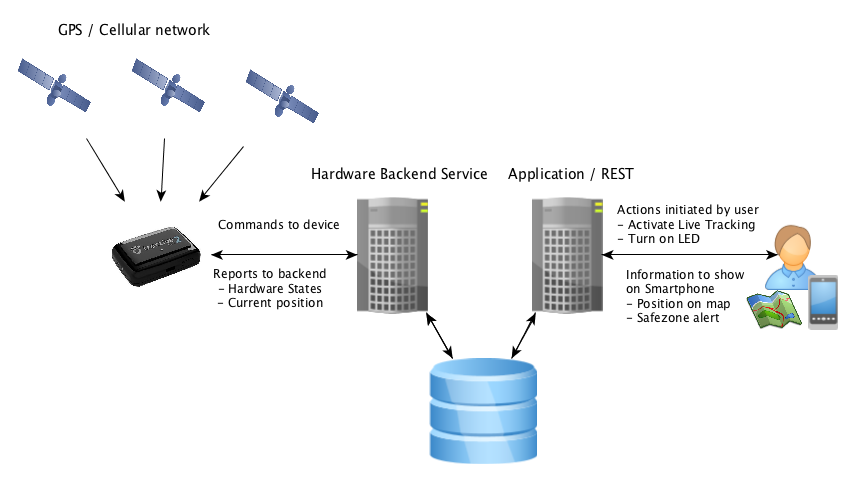
\includegraphics[width=1.0\textwidth]{img/tractiveDataFlow.png}
	\caption{Overview on communication and data flow between client and device}
	\label{fig:tractiveDataFlow}
\end{figure}

The following list outlines the essential device related data collections leveraged in the analytical part of the thesis. 

\begin{itemize}
	\item \textbf{Hardware information}: Devices usually differ when they leave the production process. Therefore some hardware details about a device are stored in its data. Following list is not comprehensive but points out attributes causing potential differences in quality for the end customer and therefore considered as valuable enough to be part of the customer satisfaction analysis process.
	
	\begin{itemize}
		\item Batch number: Devices are manufactured in mass production and assigned to a so called batch which contains devices with same configuration. If there are major changes on a devices conceptual design a new batch number gets created for the new series of devices. 
		\item Firmware version: This is the software embedded in the device. Similar to the batch the firmware gets updated as well if new features are added or problems occur. 
		\item Model number: Currently three GPS device models exist. The model of a particular device is indicated by this attribute. 
		\item Hardware edition: Tractive offers three editions which differ in their color and style but have the same hardware specs. Although not supposed as having as much quality influence as the other three attributes, it was decided to include this property in the analysis in order to investigate possible relationships between a user's taste and satisfaction. 
		\item SIM (Subscriber Identity Module) type: The communication with Tractive GPS devices is done via SMS and therefore each device has an integrated SIM card comparable to a mobile phone. Tractive uses SIM cards of three different providers to manage SMS communication. 
	\end{itemize}

	\item \textbf{Device ID reports (Device identification reports)} are sent regularly if the device is switched on and has network coverage. The ID reports contain information about the current firmware- and hardware version of the device. Since there are bug fixes and improvements on the firmware quite often, differences in service quality over time are possible. Furthermore the device identification reports allow to reason about the activity level (eg.: the number of days in use) of a customer's device.
	\item \textbf{Device position reports}: Every time a device receives a position it is sent to the backend service and in turn stored in the database. Along with the latitude and longitude of the position there is data indicating whether GPS or mobile cell network was used for localization, how strong the received signal was, as how accurate the position is classified, the timestamp when the device received the position, the time where it was stored in the database and some further technical GPS data as for instance the number of reachable satellites used for localization. The time interval in which positions are sent is configured in the hardware electronics. An exception is the live tracking feature where positions need to be sent every second to provide the customer his or her pet's location in real time. Due to fact that each position report gets stored, a lot of data is produced which makes this collection the largest data sink in the whole database. Moreover, a lot of service quality information is passed along with each position report and thus makes it a valuable data source for customer satisfaction analysis. 
	\item \textbf{Device network reports} contain data about a devices network coverage. Since the device can be used in over 100 countries worldwide each network report provides the MCC (Mobile Country Code) which indicates where the device is currently used. Prior experiences showed that network coverage sometimes varies a lot among countries which can influence satisfaction of a customer. The mobile network generation which is limited to GSM, for devices of the first generation, and UMTS, the more recent one, can have an impact on the perceived quality as well.
	\item \textbf{Device hardware reports}: These reports are usually sent along with the ID reports described before and contain different kinds of hardware states. Interesting attributes are for instance the current battery level- and voltage, temperature states, collected number of position or error and network logs for the particular device. Moreover hardware reports store specific hardware events for a point in time where they happened. Amongst others this includes valuable information as the time when the device has been switched on/off or battery is charging, full, low or at a critical level. 
	\item \textbf{Geofence reports}: Customers have the ability to define a virtual fence for their pet(s) in the mobile- or web app. If a customer's pet with a mounted device leaves or enters such a virtual fence, a geofence report with the according trigger (called in-break in case of entering the virtual fence or out-break otherwise) and source (GPS or mobile cell) is sent to the server. There it gets stored again in the database and the application initiates sending a push or mail notification (depending on the configured settings) to the customer. Both, accuracy based on the trigger source and the number of in- and out-breaks are assumed to influence customer satisfaction as it is one of the most used features among the customer base.  
	\item \textbf{Server commands}: These are commands sent due to an action initiated by the user. The most prominent server command according to the statistics is the live tracking function. If this server command is received by the device, it starts sending a new position every few seconds for a maximum defined duration threshold, which allows the user to follow his or her pet in real time on the respective client device (smartphone- or web app). Further commands enable the user to turn on/off the integrated light or trigger a sound on the device. The server commands are essential for customers of the Tractive GPS device and therefore several attributes indicating the quality are collected. For each server command the timestamps when the command was sent by the server to the device, when it was received by the device, the time of confirmation respectively cancellation as well as the duration of the command is recorded. 
	Due to the business relevance of these server commands, it was decided in March 2017 to bring this data in a different structure where detailed analysis can be done more easily than with the transactional raw data. Starting with mid of May, every new server command causes a new entry in a separate metrics collection. The calculations and persistence is done by an asynchronous job which is started one hour after a server command was created in the database. This metrics collection expands the specific server command data with useful device related data as for instance the hardware edition, batch number, SIM type or the country of usage. The meaning of these properties was already explained in the first bullet point. Furthermore, in addition to the success indication with regard to live tracking commands, the company also wanted to have information regarding time and duration of commands. Therefore, following time information gets calculated:
	
	\begin{itemize}
		\item Delay to commanded: The time it takes that a command requested by the server is received by the device. This time is only set if the command could be received by the device. The value for this attribute can be missing if the communication between backend and device did not work.
		\item Delay to confirmed: The time it takes that a command requested by the server is confirmed by the device. A command gets confirmed if the device could initiate the action (e.g. enable the live tracking function). Not all commands get confirmed. (e.g. it can happen that the device is inside a building an cannot get a strong GPS connection required for live tracking)
		\item Delay to any position: The time it takes from requesting the command by the server until the device could get a position. In order to find the time of retrieving a position, a lookup in the device position reports collection has to be done. For this type of delay there is no restriction regarding the quality of the received position. The maximum delay allowed is 90 seconds after the command was requested by the server. Only under this circumstance the usability of the live tracking function is considered as satisfying. 
		\item Delay to a new position: This delay is very similar to the one before except that it only considers new positions which were received via GPS and judged as accurate enough. 
		\item Delay to ID report: Each server command is supposed to trigger sending of an ID report as well. The maximum delay allowed is again set with 90 seconds after the command was requested by the server. 
		\item Command duration: This indicates the time the command action was enabled. This duration is only measured and stored if the command has been confirmed and terminated successfully. The exact duration hereby measured is the time passed from confirming the command by the device until the point in time where the user disabled the function. 
	\end{itemize}

	\item \textbf{Battery lifetime metrics}: Similar to a smartphone the battery lifetime is a critical component in the Tractive GPS device. If the pet is not close by and the customer wants to locate it, the battery should not be discharged. However, especially the network connection and GPS signal exhaust the battery. As Tractive also provides a position history, the device permanently (with regular gaps) tries to fetch a new position. With live tracking enabled battery suffers even more. Depending on the intensity of usage, the battery lifetime varies. This should be expected by customers but despite that fact battery lifetime varies between GPS devices. Since battery lifetime is considered as critical, it was decided to create a new collection suitable for detailed analytics of battery lifetime among devices analogically to the server command metrics. In addition to some hardware information as the model number and hardware edition this collection stores battery cycles, based on the device hardware reports, which were explained in more detail the fourth bullet point. Each time a hardware report with status indicating full battery is received from the device, an asynchronous job is executed to calculate the information for the previous battery cycle, starting with the highest reported battery level and ending with the lowest one before recharging the device again. Due to the complexity of reliably calculating time for a battery cycle threshold were defined to categorize a battery cycle. In order to characterize a cycle as full, the highest battery level reported has to be at minimum 90\% and the lowest one at maximum 10\%. Moreover the device should not have reported any shutdown since this would distort the result. As of 30.11.2017 17:54, 45.32\% of all reported valid battery cycles were characterized as full ones. Despite the fact that durability of a battery in an electronic device is unreliable, this thesis considered only full cycles as representative to reason about average battery lifetime of a tracker as interpolation calculations from incomplete cycles would lead to invalid results. Due to the reason that recording those battery cycles was implemented later during the empirical work, the author had to notice that not as much data as desired is available for the average battery lifetime calculation of devices. This restriction had to be considered accordingly during the analysis part. 
\end{itemize}

\subsubsection{Notification related data} 
Notifications play an essential role for Tractive customers, as for instance the information whether a pet has left a defined virtual fence can be crucial for customers. The assumption made in this thesis relies on the fact that reliability of notification delivery either via mail but even more important via push notification on the smartphone has an influence on customer satisfaction. Customers of the Tractive GPS smartphone app can receive a palette of different push notifications. Following listing briefly summarizes the notification types which the author considered as potentially influential.

\begin{itemize}
	\item \textbf{Geofence Notification}: The opportunity to define a virtual fence for his or her pet is one of the mostly used features among Tractive GPS customers. As a result it is important to get a notification if a pet leaves or enters such a virtual fence. This is represented by a Geofence Notification which contains the affected device identifier as well as the information whether the pet left or entered the virtual fence. According to the importance, this type of notification is considered to be of highest priority. 
	\item \textbf{Hardware battery notification}: As the device is mounted on the collar of a pet and the customer most of the time is not close by, it is a relief to get updates about the battery state. In addition to the device identifier, a particular battery state of an predefined enumeration of states is stored.
	\item \textbf{Resource notification}: In terms of the use case of Tractive a resource can be of different type whereby an image is the relevant one for this notification type. Next to the Tractive GPS app which is the main product for customers of a GPS device, there are other apps to use. Users can for instance share their photos with other Tractive users or photos can be liked or commented on from the Tractive community. As such notifications are not direct quality indicators, they are ranked low on importance.
	\item \textbf{Hardware alert notification}: These notifications are sent based on sensor measurements of the hardware device. Exposed sensor values are temperature and mount state of the device. A customer should receive a notification if the temperature of the device is too high respectively low as well as when the device gets unmounted from the collar. As these hardware alerts are only present for a specific version of the GPS device, there is little data available for analysis. Thus, these notifications are considered as low priority when it comes to customer satisfaction.
\end{itemize}

Every notification sent from the system is stored in the database with the information, depending on the specific type, described in the previous listing along with user data. As a consequence it can be followed which and how many notifications of a specific type a customer has received until a point in time. 

In addition, any mail- and push notification results are stored in according log collections. 
Especially for time critical notifications like geofence notifications, the time passed between the event has been triggered by the device and received as notification in the push bar of the smartphone would be of big interest. Since push notifications are sent via a publish/subscribe message bus and later through the respective push service of iOS and Android, there is currently no mechanism implemented to measure and store this overall time. As a consequence, the available notification data is limited to the bare number of received notifications in a specific interval. 

\subsubsection{Customer service related data}
Tractive advertises a first-class customer service which about a third of customers of a GPS device actually make use of. An extracted statistic from the database shows that since February 1st, the date where Tractive started to sync support contacts to the database, 34.42\% of new customers who activated a device had at least once contact with the customer support. These numbers clearly emphasize the importance of a good and responsive customer service. As explained in section \ref{sec:custSatisfactionDefinition} when illustrating the model from \cite{johnson2001evolution}, customer service is assumed to contribute to the customer satisfaction complex. 

In order to bring more structure in the collected information, Tractive employs a customer support service tool called Zendesk® which is the central place for desires, complaints and support requests. Instead of traditional email, a customer can send a support request via a help center web page. As result, a support ticket in Zendesk® gets created which can then be handled by support employee of Tractive. This ticket based approach makes the support team more efficient. In addition, it allows a better data integration and has the advantage that all collected information regarding particular support tickets is stored transparently in Zendesk® and can be retrieved if needed.

From a technological perspective every update on a support ticket is synced with the backend service and stored in the database. Moreover, Zendesk® provides a comprehensive REST API to query details of a specific ticket. As particularly interesting the author considered the opportunity to query ticket metrics provided by Zendesk®. Following listing briefly outlines the ones considered as valuable in terms of quality indication for customer support \cite{zendeskWeb}.

\begin{itemize}
	\item \textbf{Ticket count}: The number of tickets a customer opened.
	\item \textbf{Requester waiting time}: The time a customer has to wait in- and outside of business hours until he or she receives the first answer.
	\item \textbf{Reopens}: Indicates how often a ticket was reopened. Reopening a ticket usually happens if the problem of a customer reappeared after the support employee closed the ticket as resolved.
	\item \textbf{Resolution time}: The time it takes to fully resolve a customer's incident in- and outside of business hours. This covers the time from opening a ticket for the first time until it is closed an not reopened again. 
	\item \textbf{Replies}: The total number of times a ticket was replied to.
\end{itemize}

The mentioned metric attributes can be queried for every ticket in the system. Before being able to query these metrics, the tickets of a customer can be found via their email address which is needed while registering a Tractive account. 

\subsubsection{Subscription related data}
Every customer who purchased a Tractive GPS device has to activate it in order to be able to use it. This device activation results in a subscription which enables recurring payments for the tracker usage comparable to a mobile phone contract. Tractive offers payment plans differing in their type, which can either be "basic" or "premium", and the payment interval, which can be monthly, annually or biennially. In addition, customers have the opportunity to opt in for a device insurance to get a free substitution device in case the first one gets lost or breaks accidentally. Customers can cancel their contract any time they want and also have to possibility to change their payment plan at any point in time during their relationship with the company. This can be done in form of upgrading or downgrading the subscription type or changing the payment interval. Based on previous work regarding customer satisfaction theories as described in section \ref{sec:custSatisfactionDefinition}, price and costs are considered as influential factors for customer satisfaction. 

The whole payment and subscription related data of customers is spread over several collections in the database. From a thesis' perspective the focus is put on the subscription information which is the actual interface between a customer and his or her device. The type and payment interval as well as the information whether a customer added the device insurance to his subscription were assumed as most influential factor. Tractive on the one hand offers a cheaper price if the customer chooses to subscribe for a year or even two years instead of just a month and on the other hand advertises more features to premium customers. As a consequence both customer expectations and perceived quality should vary based on his or her choices.

\subsubsection{Other relevant data}
In addition to the categorized data sources, the search yielded some more data attributes among different collections which are worth to investigate in more detail during the analysis part. Since this data does not fit together in any of the defined categories, the thesis groups them together in this section. 

As interesting metric, the number of times a customer opened the Tractive GPS smartphone app in a specific time interval, was considered. Although this information is stored in a separate mobile events collection, the data is not highly reliable as the sent events vary between iOS and Android. Moreover, there are different events, like app\_foreground and app\_startup on Android, where it is later not possible to be sure what behavior the user really showed. As a result, these events are only vague numbers and have to be handled with care. Next to the Tractive GPS app, some other mobile apps from Tractive are available in the according app stores. This information is supposed to give more insights into the engagement of a customer in the Tractive ecosystem and his or her appreciation of the brand. 

The importance of social media marketing definitely plays a major role at Tractive. Customers love to share photos of their pets to other people and thus Tractive also employs their own photo platform. Users can upload photos as well as comment and like photos of others. Although social activities do not directly emerge as predictor from the customer satisfaction model introduced in section \ref{sec:custSatisfactionDefinition}, this thesis wants to check possible correlations and therefore included available data in the analysis. It was found out that the number of resources liked and commented on associated with a user can be derived from available data. As no published research work focusing on such a relationship could be found during literature research, it was worth to take a look on possible correlations as part of the analysis. 

\subsubsection{Data not considered as relevant}
\label{sssec:excludedData}
Based on the relevant data sources introduced in this chapter so far, the attentive reader can see that there is already a lot of data which has the potential to make a difference in terms of customer satisfaction. However, to make clear why these choice were made when searching for relevant data sources, this section exemplarily outlines attributes which did not make it in the analysis part. 

Since Tractive is operating world wide, customers come from different countries and speak various languages. Geographical- and demographical data, like country, language or gender is considered as static and does not reflect a customer's behavior. Customers can assign a pet to their tracker and enter detailed information about their pet like type, name, weight, height or breed. Despite the fact, that this information can be valuable for the company in order to get more insights about the type of pets the device is often used for, it is not topic of usage behavior and thus not considered as relevant for customer satisfaction in this thesis. 

Lastly, it is important to notice the general limitation of customers whose data is used during analysis, as only those who activated at least one GPS device, are considered. Other users who have registered and probably use some other Tractive app without a GPS device will not be considered at all in this thesis. On the one hand, there is too little data available for them and on the other hand these customers are topic of customer- acquisition instead of retention. Moreover, some customers own more than one device which would produce problems when data is tied to the user ID and not to the particular customer-device relation. An example would be the app usage where no separation based on the device can be made. It could be for instance the case that a user often opens the app to locate one of his or her pets but is not interested in the other activated devices. When comparing this number with device specific information the matching would lead to wrong results and as a consequence wrong input for the analysis part. Since the customer base of Tractive is big enough, the analysis only considers customers with one activated device which fixes the outlined problem and prevents distorted results. 

\section{Implementation of a data extraction tool}
\label{sec:extractionTool}
After identifying relevant data sources and matching them to specific collections and attributes in the NoSQL database, the first major technical task was the implementation of a program to extract this data and bring it in a format which allows analysis by a statistical program. 

In contrast to a relational database, MongoDB uses JavaScript for querying and manipulating data. Principally data can be queried via the MongoDB shell which comes in handy when doing standalone queries. However, for the planned amount of data extraction a lot of querying has to be done among different collections. In order to connect results and manipulate them accordingly to prepare it for the analysis, more logic was required. Thus, a data extraction program was implemented in JavaScript which uses the NodeJS MongoDB driver to connect to the database as illustrated in code listing \ref{lst:mongoConnect}.

\begin{lstlisting}[caption={Connecting to the database via MongoDB NodeJS driver}, label={lst:mongoConnect}]
var connection = {};

function createDbConnection(url, port, database, cb) {
	MongoClient.connect('mongodb://' + url + ':' + port + '/' + database, function (err, db) {
		if (err) {
			throw err;
		}
		if (database === 'tractivedb') {
			connection.tractivedb = db;
		} else {
			connection.metrics = db;
		}
		cb(null);
	});
}
\end{lstlisting}

The implementation leverages the powerful aggregation framework of MongoDB for most of the collections where data should be collected. This aggregation framework provides a palette of operators for grouping and aggregating data which makes it easier to perform certain queries which are standard in SQL (Structured Query Language) but hard to do with a NoSQL database. The programmer can specify a pipeline of operations where the intermediate result is passed top-down. Especially the rather huge amount of promising attributes in the device related data collections made it necessary to make querying functions generic and reusable. The code snippet illustrated in listing \ref{lst:aggregationServerCommands} shows how to query the average of a certain metric of an arbitrary server command for a device used within a defined time interval. As a result this method can be used for different server commands not matter whether it is the live tracking command or led switcher. Plus it can be reused to calculate for instance the average of successfully- , canceled -, or terminated commands which makes the function quite flexible to use. 

\begin{lstlisting}[caption={Aggregation query on server command metrics collection}, label={lst:aggregationServerCommands}]
var COLLECTION = 'server_command_metrics';

function queryServerCommandMetricsForTracker(commands, cmdStatistic, startDate, endDate, trackerId, cb) {
	var matchCriteria = {};
	matchCriteria[cmdStatistic] = {'$exists': true};
	matchCriteria['msg_name'] = {$in: commands};
	matchCriteria['mode_on'] = true;
	matchCriteria['device_id'] = trackerId;
	matchCriteria['requested_at'] = {'$gte': startDate, '$lt': endDate};
	
	var groupStage = {_id: '$device_id'};
	groupStage[cmdStatistic] = {$avg: '$' + cmdStatistic};
	
	var pipeline = [
		{'$match': matchCriteria},
		{'$group': groupStage}
	];
	
	db.aggregate(db.getMetricsDbConnection(), COLLECTION, pipeline, cb);
}
\end{lstlisting}

The previous code snippet shows that the execution of all those MongoDB queries is asynchronous as indicated by the last parameter of the function called "cb". Every asynchronous function in the data extraction program is handled by a callback which returns either an error if the operation failed or the respective result object. Handling asynchronous results in JavaScript quickly gets confusing and increases maintenance effort due to the nesting of callback functions. Since some of the queries require as input the result from a previous query, the implementation makes use of the async library to handle the control flow of asynchronous function executions. How this can look like in JavaScript is shown in listing \ref{lst:asyncExmaple}.

\begin{lstlisting}[caption={Example of using async for handling the control flow of asnychronous database queries}, label={lst:asyncExample}]
function getAppUsagesForUsers(userIds, startDate, endDate, cb) {
	async.series({
		clientIds: queryClients
	}, function (err, result) {
		async.waterfall([
			async.apply(db.createConnection, 'tractivedb_metrics'),
			async.apply(queryAppUsagesForUsers, userIds, 
			util.getObjectIdsAsStringArray(result.clientIds), startDate, endDate)
		], function (err, appUsages) {
			cb(err, appUsages);
		});
});
}
\end{lstlisting}

The illustrated JavaScript example provides an insight how finding the app usage of users is implemented. On the top level there is an asynchronous function to retrieve all available clients (i.e. the different Tractive apps). The waterfall function is used to pass the resulting connection object from the callback of the createConnection method to the actual function which queries the app usage of customers. With async.apply additional parameters can be passed to the respective function. 

To construct pairs of attribute vectors, the query results represented as JSON objects available in memory have to be combined correctly to make them comparable by statistical methods. In order to analyze for instance a relationship between the average success rate of server commands and the number of times the customer opened the Tractive apps, a common property has to be used to merge the results. This reference property in most cases is the unique ID of the registered user or, if not available in one of the two data sets to merge, the unique device ID. As already mentioned in section \ref{sssec:excludedData} only customers with one device are present in the samples which allows to safely merge based on both properties. With regard to the upcoming section which will shed light onto the first analysis approach, the resulting feature vectors finally were printed to separate CSV files which is the most common file format and interpretable by any statistics software.

\section{Hypotheses-driven approach to gain knowledge about interrelationships in data}
\label{sec:hypothesesDriven}
Based on the prepared data, analysis work started with a top-down approach as described in section~\ref{ssec:topDown}. The aim was to get an understanding which of the extracted data related to customer behavior is expressive enough to be considered as influential factor for customer satisfaction. Hypotheses were explicitly defined and either verified or falsified by statistical measurements. It was planned to use results if they are promising to build a framework which allows predicting the satisfaction level of other customers. 

\subsection{Choosing target data approximating Customer Satisfaction}
While section~\ref{sec:dataSources} explored the available data sources to identify those which are assumed to be predictors for customer satisfaction, the work explained in this section analyzed data with regard to actual correlations. Due to the lack of explicit customer feedback, the author had to overcome this difficulty by choosing implicit data as target variable for customer satisfaction. This data should be expressive enough to distinguish between satisfied and dissatisfied customers. The author proceeded by finding behavioral patterns, customers would follow if they feel pleased or disappointed and came up with following collected data:

\begin{itemize}
	\item Recurring service active or canceled: The assumption hereby is that satisfied customers will keep their service where they pay monthly, yearly or biennially and are therefore able to use the device anytime. Dissatisfied customers are vulnerable to cancel the service and end the relationship with the company after the current payment interval has ended. These thoughts are based on the theory of relationship between customer satisfaction and loyalty outlined in section \ref{sec:problem}.
	\item Increased or diminished app usage: The assumed behavioral property resulting from (dis)satisfaction is that customers increase respectively diminish the usage of the smartphone app. According to analytics data, the Tractive GPS app for iOS and Android is most important for customers of a Tractive GPS device. As a result of good user experience it is expected that customers get more satisfied and therefore use the app more often.
	\item How many days a GPS device is in use: The device ID reports, explained in more detail in section~\ref{sssec:deviceRelatedData}, can be seen as an activity indicator when aggregated over a period of time. The thesis considered the number of days the device sent ID reports as a meaningful number related to increased of decreased satisfaction.
\end{itemize}

\subsection{Formulation of Hypotheses and solving analysis problem}
The upcoming paragraphs provide a more detailed insight into the procedure of defining hypotheses and the appliance of statistical tools to verify respectively falsify them. Following, a sample of executed analysis tasks is exemplarily outlined. 

\subsubsection{Live tracking feature as customer churn indicator}
This first analysis done in the implementation part of this thesis is based on the relationship between customer satisfaction and loyalty. Therefore the thesis differentiated between the service status "active", which indicates that a customer is paying on a recurring basis, and the service status "terminated", which indicates a manual service cancellation by a customer. This implies the fact, that this task relies on binary categorical data. The analysis goal was then stated as following: Does Live Tracking success influence service termination behavior?

\begin{enumerate}
	\item Hypotheses
	\begin{description}
		\item[H0] There is no significant difference in service termination behavior between customers who belong to the group of bad live-tracking users and customers who belong to the group of good live-tracking users.
		\item[H1] There is a significant difference between these two groups.
	\end{description}
	\item Analysis objects
	\begin{itemize}
		\item Live Tracking Server commands related to a specific device
		\item Service status of customers
	\end{itemize}
	\item Analysis problem
	\begin{itemize}
		\item Select representative sample and split it up into two groups to compare, namely a treatment and control group. It is important to exclude any other influencing factors as best as possible and therefore define common base data shared among both groups. 
		\item Choose a suitable sample size
	\end{itemize}
	\item Analysis solution: Statistical test which should check whether the Null-hypothesis can be rejected and thus statistical significant difference can be shown. The analysis was done on 17.04.2017. 
	\begin{itemize}
		\item Group selection: The first group contains random customers suffering from bad live tracking which was defined by an overall success rate below 70\%. In contrast, the control group consisted of customers with a success rate greater or equal than 80\%. These thresholds were set according to experience in customer support where complaints from users regarding live tracking usually show success rates around this threshold. As common base data only users from Germany who own one Tractive GPS device and have a subscription of type basic with a monthly payment interval, which was created before 01.10.2016 and is at least valid until 01.10.2016, were considered. 
		\item Choosing a suitable sample size: The sample size for the two groups was estimated based on findings of \cite{campbell1995estimating}. Regarding statistical significance a widely used $\alpha$-error of 5\% was used while a $\beta$-error of 10\% should reduce the probability of false-negative results, meaning non-rejection of H0 although it could have been rejected. Since a statistical significant result does not necessarily say something about expressiveness of the computed result, a minimal relevance level had to be set for choosing an appropriate sample size. A 20\% decrease of active subscriptions due to bad Live Tracking was considered as relevant. Picking the right number from the sample size table proposed by \cite{campbell1995estimating} yielded a size of 79 items group, or 158 in total. 
		\item Querying data: At the time where this particular analysis was conducted no analytical view on the server command metrics was available and therefore the procedure was to calculate those metrics for the devices under consideration manually. Therefore the implementation fetched a random sample of subscriptions with the specified size, either of status "active" or "terminated" with the described common data. Based on the device ID reference, server commands of type "Live Tracking" within the given time period were filtered and the success rate averaged. Based on the output data a post-processing step provided a simple 2x2 table which is illustrated in~\ref{tab:binaryLtData}. 
		
		\begin{table}[]
			\centering
			\resizebox{\textwidth}{!}{%
				\begin{tabular}{|l|l|l|}
					\hline
					\multicolumn{1}{|c|}{\textbf{}} & \multicolumn{1}{c|}{\textbf{Service status = ACTIVE}} & \textbf{Service status = TERMINATED} \\ \hline
					\textbf{Good Live Tracking}     & 54                                                    & 8                                    \\ \hline
					\textbf{Bad Live Tracking}      & 43                                                    & 19                                   \\ \hline
				\end{tabular}%
			}
			\caption{2x2 table showing influence of Live Tracking on service status}
			\label{tab:binaryLtData}
		\end{table}
		\item Statistical test to verify or falsify H0: There are different statistical tests for binary data whereby Fisher's exact test is proposed as most suitable for a rather small sample size as it was in this case \cite{raymond1995exact}. The test works based on a 2x2 table as input and calculates a 95\% confidence interval indicating where the true odds ratio lies. The odds ratio is an often used value when analyzing binary data and states the relative probability than an event occurs against that it does not occur \cite{bland2000odds}. The Null-hypothesis in Fisher's exact test can be rejected if the confidence interval does not include the odds ratio 1. Then it is safe to claim that there is a difference between the two sample groups under consideration. The open source statistic program package R was used to execute the Fisher exact test, as illustrated in listing \ref{lst:fisherTest}, for the 2x2 table. 
		
		\begin{lstlisting}[caption={Execution of Fisher's exact test in R}, label={lst:fisherTest}]
		m <- matrix(c(54, 8, 43, 19), 2, 2)
		fisher.test(m)
		\end{lstlisting}
		The result yielded a confidence interval of $[1.105933, 8.604534]$ which indeed allows rejecting H0. Based on this statistical experiment it is thus valid to say that there is a statistical significant and based on the minimum of 20\% difference in terminations between treatment and control group also a relevant result.
		\item Interpreting the result: This data analysis confirms the expected importance of the live tracking function for Tractive customers since terminating an active service is equal to ending the relationship with the company and can therefore be considered as a last resort in case of dissatisfaction. As a result it can be stated that live tracking success rate qualifies as potentially promising feature for customer satisfaction. 
	\end{itemize}
\end{enumerate}

\subsubsection{Abnormally canceled live tracking as indicator for app usage}
\label{sssec:liveTrackingAppUsage}
This example investigated the potential relationship between live tracking commands, which were not canceled on purpose by the customer, and the app usage.  

\begin{enumerate}
	\item Hypotheses
	\begin{description}
		\item[H0] There no significant difference in the app usage between customers with a higher canceled LT rate and the ones with a lower rate.
		\item [H1] There is a difference in the app usage between those two groups. 
	\end{description}
	\item Analysis objects
	\begin{itemize}
		\item Server command metrics collection
		\item App Events collection containing app startup and app foreground events
	\end{itemize}
	\item Analysis solution
	\begin{itemize}
		\item Choose a suitable sample size: For an appropriate choice the width of the confidence interval, where the true correlation coefficient of the population lies, was considered. The author decided on 0.1 as its width for the experiments to ensure a high precision. Since the app usage was not considered as a direct measurement of a customer satisfaction value, a sample correlation coefficient of 0.4 was determined as relevant. Based on these parameters and the research of \cite{moinester2014sample}, a sample size of 1086 could be derived for the correlation analyses. 
		\item Select sample users: The selection was done by randomly skipping users. Since a few users did not execute any server command with the selected time period, the sample size was automatically reduced by the program to 1065. The output of this selection stage contained user- and device ids.
		\item Query data to compare: The sample users fetched in the previous stage were used as input parameter for the function which fetches the number of app foreground events within a selected time period for the current user under consideration. 
		\item Match data based on user ID: The data collected was stored in JSON (Javascript Object Notation) arrays in-memory. A matching function finally generates the input vectors for the subsequent statistical calculations, by matching the nested JSON objects via the user id and writing data to one CSV file each. 
		\item Use correlation analysis to reason about linear relationship: After finishing the querying part, the data was ready for correlation analysis. Therefore the statistical open source program package R was used to calculate a Bravai-Pearson correlation coefficient. The calculation part is illustrated in listing \ref{lst:pearsonCorrelation}. 
		
		\begin{lstlisting}[caption={Calculation of pearson correlation and statistical test in R}, label={lst:pearsonCorrelation}]
		cmdCancelleDrate = read.table("hypo-tests/data/cmdCancelledRate.csv", sep = ',')
		appUsages = read.table("hypo-tests/data/appUsageCancelled.csv", sep = ',')
		cor(cmdCancelleDrate, appUsages)
		\end{lstlisting}
	\end{itemize}

	The scatter plot shown in figure \ref{fig:canceledvsAppUsage} does not look promising with regard to any kind of linear relationship between the abnormally canceled live tracking rate and the app usage. 
	
	\begin{figure}
		\centering
		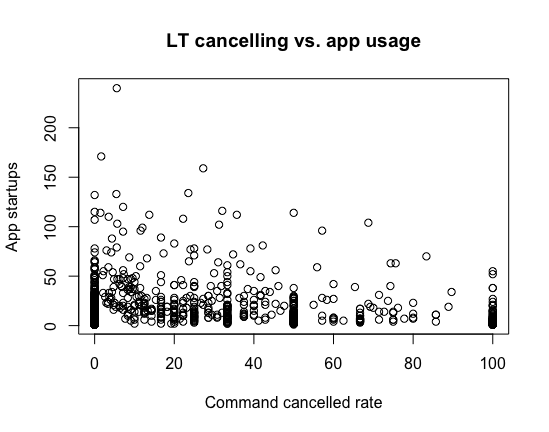
\includegraphics[width=0.8\textwidth]{img/LT_cancelled_rate_vs_app_usage.png}
		\caption{Scatterplot - Canceled rate vs. app usage}
		\label{fig:canceledvsAppUsage}
	\end{figure} 
	
	The calculated Pearson correlation coefficient is $r = -0.0420426$. 
	This result indicates a negative linear correlation as it was expected by the null hypothesis, which in essence claims that a higher rate of canceled server commands leads to a diminished app usage. However, the result confirms the visualization in the scatter plot from before as it is close to zero.
	In order to formally prove the hypotheses under test, the Pearson's product moment correlation test was applied on the two data rows. This test calculated a 95\% confidence interval to verify whether the Pearson correlation coefficient is statistically significantly different than $0.0$. (indicating no linear relationship at all) Listing \ref{lst:pearsonCorrelation} shows how this was done in R. 
	
	\begin{lstlisting}[caption={Pearson correlation test in R}, label={lst:pearsonCorrelation}]
	cor.test(cmdCancelledRate, appUsages)
	\end{lstlisting}
	
	Following, the result of this correlation test is shown.
	$
	alternative hypothesis: true correlation is not equal to 0
	95 percent confidence interval:
	-0.10185605  0.01807374
	$
	As a result it can be stated that here is no significant relationship between these two data attributes. 
\end{enumerate}

\subsubsection{Signal Strength vs days in use}
The third example concluding the exemplary listing of hypotheses regarding customer satisfaction, had the goal to investigate whether the quality of the received signal from the telecommunication network influences the activity level of the tracker determined by a customer's usage behavior. For the signal strength an available indicator are the RSSI (Received Signal Strength Indicator) values from the GSM network (Global System for Mobile Communications). These RSSI are stored inside a position report. Due to the reason that customers also sometimes try to locate the device when their pet is indoor, it can happen that the RSSI value of a position report is good although there is no GPS signal available and as a result the location is inaccurate. Therefore it was important to only consider RSSI values where the used sensor was GPS. The activity level of a device can be queried via the ID reports. The most common metric used at Tractive's business is the number of ID report aggregated per day. (i.e. the number of days the device was in use) Following is a summary of the analysis executed. 

\begin{enumerate}
	\item Hypotheses
	\begin{description}
		\item[H0] There is no significant difference regarding the days a device was in use between customers with a higher average RSSI and the ones with a lower one.
		\item [H1] There is a difference in the days a device was in use between those two groups. 
	\end{description}
	\item Analysis objects
	\begin{itemize}
		\item Device position reports collection
		\item Device ID reports collection
	\end{itemize}
	\item Analysis solution
	\begin{itemize}
		\item Choose a suitable sample size and sample users: Selecting the sample of users for this analysis task was chosen based on the thoughts from the previous analysis task outlined in \ref{sssec:liveTrackingAppUsage}. As a result, 1086 users could be randomly selected.
		\item Query data: Since the data extraction tool was implemented in a generic way it provides a function to query any average value for the different hardware attributes which come along in a position report. The average GSM RSSI value for GPS based position reports was queried and stored in a JSON array. The second part to prepare the data was querying the device ID reports grouped by the ID of the device with an $dayOfMonth$ aggregation over the report time. Finally, the sum of documents retrieved are summed up for each device which yield the number of days in use.  
		\item Match data based on device id: The base matching function to merge the RSSI data with the days in use was reused here with the exception of taking the device ID as matching parameter because the user ID was not available in the considered collections. 
		\item Similar to the previous analysis task, this example also deals with two continuous numeric data vectors and therefore the Bravai-Pearson correlation coefficient could be used as statistical relationship measurement. 
	\end{itemize}
	\item [Results] 
	The scatter plot illustrated in figure \ref{fig:gsmRssiVsDaysInUse} shows a random distribution of points indicating no relationship between the GSM RSSI value and the number of days the GPS device was in use within the given time period. 
	
	\begin{figure}
		\centering
		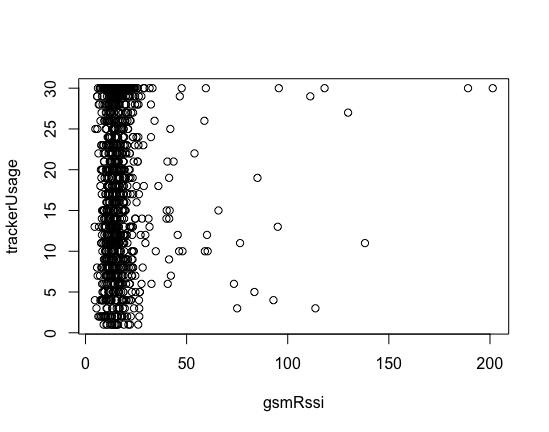
\includegraphics[width=0.8\textwidth]{img/gsmRssiVsTrackerUsagePlot.png}
		\caption{Scatterplot - GSM RSSI vs. Days in use}
		\label{fig:gsmRssiVsDaysInUse}
	\end{figure} 
	
	Calculated Pearson correlation coefficient: $r = 0.01835016$. 
	Analogically to the previous analysis tasks, the Pearson's product moment correlation test was calculated and yielded as a result that the Null hypothesis cannot be rejected since the calculated 95\% confidence interval includes the value $0.0$. The essential result from R is shown below.
	$
	alternative hypothesis: true correlation is not equal to 0
	95 percent confidence interval:
	-0.04118162  0.07775211
	$
\end{enumerate}

\subsection{Evaluation of approach and derived decisions}
The first analysis task for a randomly selected sample of subscriptions yielded a statistical significant and clinical relevant difference between users tending to behave loyal in terms of staying active subscribes and users tending to cancel their subscription based on the live tracking success rate. The asymptotic Chi-Square test as well as Fisher's exact test supposed to reject the Null hypothesis which confirmed the initial assumption that the live tracking success rate is a critical business factor for Tractive. However, due to complexity regarding the aggregation queries and hypothesis test possibility, this statistical test only considered two groups of subscription states, namely "active" and "terminated". Therefore payment failures and as a result expired- as well as paused services were not considered. In the following hypotheses driven tests several correlation coefficients between a given behavior metric and an assumed customer satisfaction driver, like the app foreground events or the number of a GPS device's usage days, were calculated. For none of them the author of this thesis could derive any further influential factor for customer satisfaction. One of the major issues identified is the single implicit metric used to explain customer satisfaction. The lack of explicit feedback from a sample of customers introduced big difficulties to see customer satisfaction through the eyes of the proposed base model from \ref{fig:satisfactionModel} introduced in section \ref{sec:custSatisfactionDefinition}. customer satisfaction is a much more complex construct and it turned out to that the app usage or usage days of the GPS device are not sufficient to make a promising statement. Although \cite{kim2013study} came to the conclusion, after their survey results analysis, that mobile usage of customers in nowadays smartphone dominated world has a major influence on satisfaction, their proven hypotheses contained mobile engagement motiviation as primary factor. This engagement can be characterized as a three dimensional model consisting of the functionality of a mobile app driving a users efficiency to accomplish tasks, the ease of use and entertainment factor and a social component indicating whether it is possible to connect with friends via the app \cite{VARNALI2010144}. The results of \cite{kim2013study} furthermore show that mobile engagement and perceived value can create a basic satisfaction level for a user which in turn leads to more engagement motivation and as a result increases satisfaction. This mobile engagement- and satisfaction model is not well represented by the single dimension of app opening events. As a result the data analysis tasks explained in the previous part of this thesis underperformed.

The difficulty in finding a representative metric, which provides a better chance to get more accurate results, from the collected data at Tractive led to the following decision. In conjunction with the company the author decided to design a customer survey which will be sent to users who purchase and successfully activate a GPS device. The survey asks them a few questions to find out how satisfied they are with the product. An essential part was the type, formulation and number of questions to ask the customer in order to get representative knowledge. The goal was to incorporate the gathered data back into the software system, extract potentially satisfaction driving features as mentioned in section \ref{sec:dataSources} for those customers and learn from this data. Identified relevant data sources should be reused and further extended in this part of the thesis but the approach should be a different one. The upcoming chapter \ref{ch:dataDriven} will shed more light onto the approach and describes the implementation in greater detail. 




 

